\begin{landscape}
\chapter{Листинги}
\section{Конфигурационный файл параметров сети Modbus}\label{app:sec:modbus_tag}
    \lstinputlisting[
        language=MyXML,
        caption=Конфигурационный файл для описания множества контроллируемых параметров по промышленному протоколу Modbus
            из раздела \ref{sec:modbus_tag}. Файл разметки приведен в листинге \ref{lst:modbus_tags_example_configs}.,
        label=lst:modbus_tags_example]
            {Dissertation/listings/xml/modbus_tags_example.xml}
\end{landscape}

\section{Конфигурация сценария}\label{app:sec:modbus_scenario_example_diagram}
\lstinputlisting[
    language=MyXML,
    caption=Конфигурационный файл примера сценария развития событий (см. рисунок \ref{fig:modbus_scenario_example_diagram}).,
    label=lst:modbus_scenario_example_diagram]
        {Dissertation/listings/xml/modbus_tags_example_scenario.xml}

\begin{landscape}
\section{XML схемы}\label{app:sec:xsd}
    \lstinputlisting[
        language=MyXML,
        caption=Схема разъметки конфигурационного файла из листинга~\ref{lst:modbus_tags_example}.,
        label=lst:modbus_tags_example_configs]
            {Dissertation/listings/xsd/modbus_tags_configs.xsd}
    
    \lstinputlisting[
        language=MyXML,
        caption=Схема разъметки конфигурационного файла из листинга~\ref{lst:modbus_scenario_example_diagram}.,
        label=lst:modbus_tags_scenario_configs]
            {Dissertation/listings/xsd/modbus_tags_scenario_configs.xsd}        
\end{landscape}

\begin{landscape}
    \section{Онтология модели АНПА}\label{app:sec:anpa_owl}
    \lstinputlisting[
        language=MyXML,
        caption=Описание онтологии на языке \texttt{RDF}.,
        label=lst:model_anpa_owl]
            {Dissertation/listings/owl/anpa_2.owl}
\end{landscape}


\chapter{Свидетельство о государственной регистрации программы для ЭВМ}\label{app:sec:registration}
\begin{figure}[hb]\begin{center}
    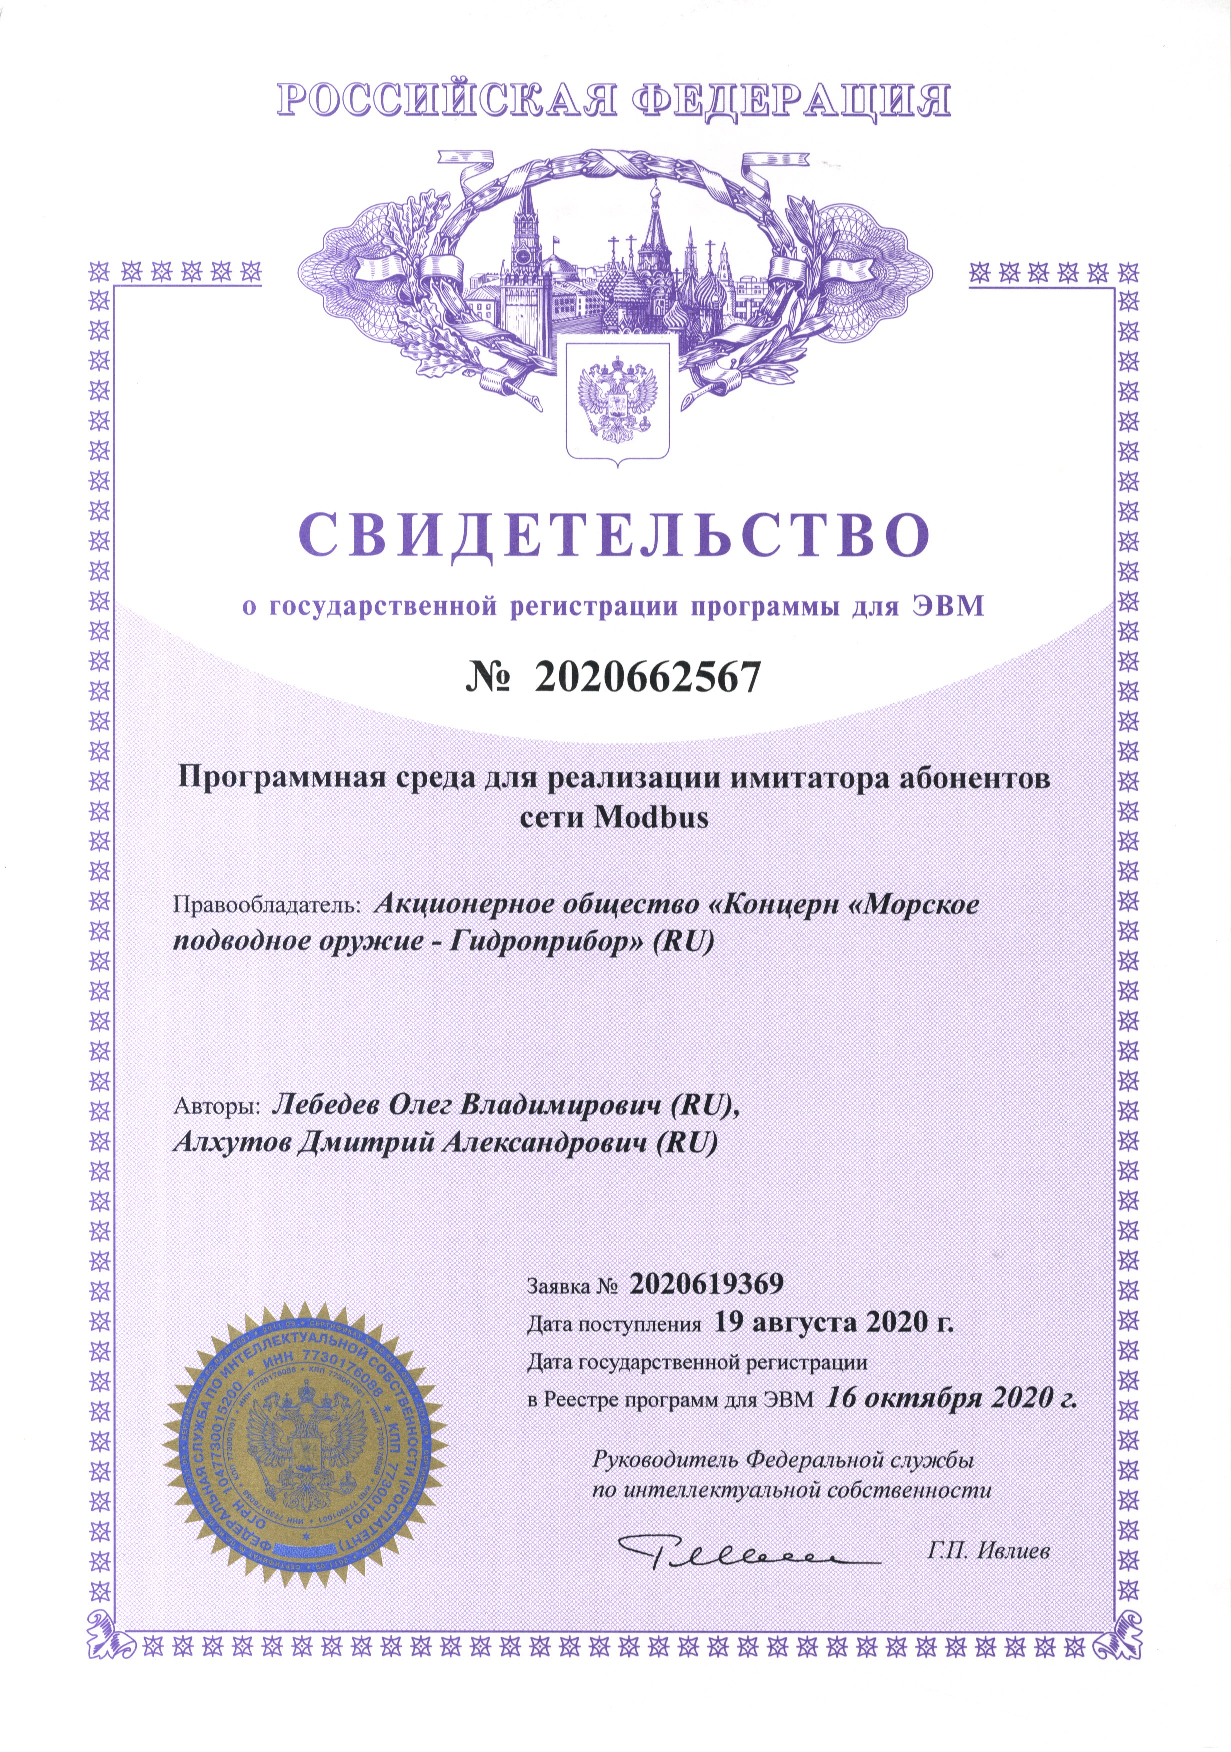
\includegraphics[height=.75\textheight, keepaspectratio]{registration.pdf}
    \caption[Свидетельство о государственной регистрации]
        {Свидетельство о государственной регистрации программы для ЭВМ.}\label{app:fig:registration}
\end{center}\end{figure}


\chapter{Акт о внедрении}\label{app:sec:implementation}
\begin{figure}[hb]\begin{center}
    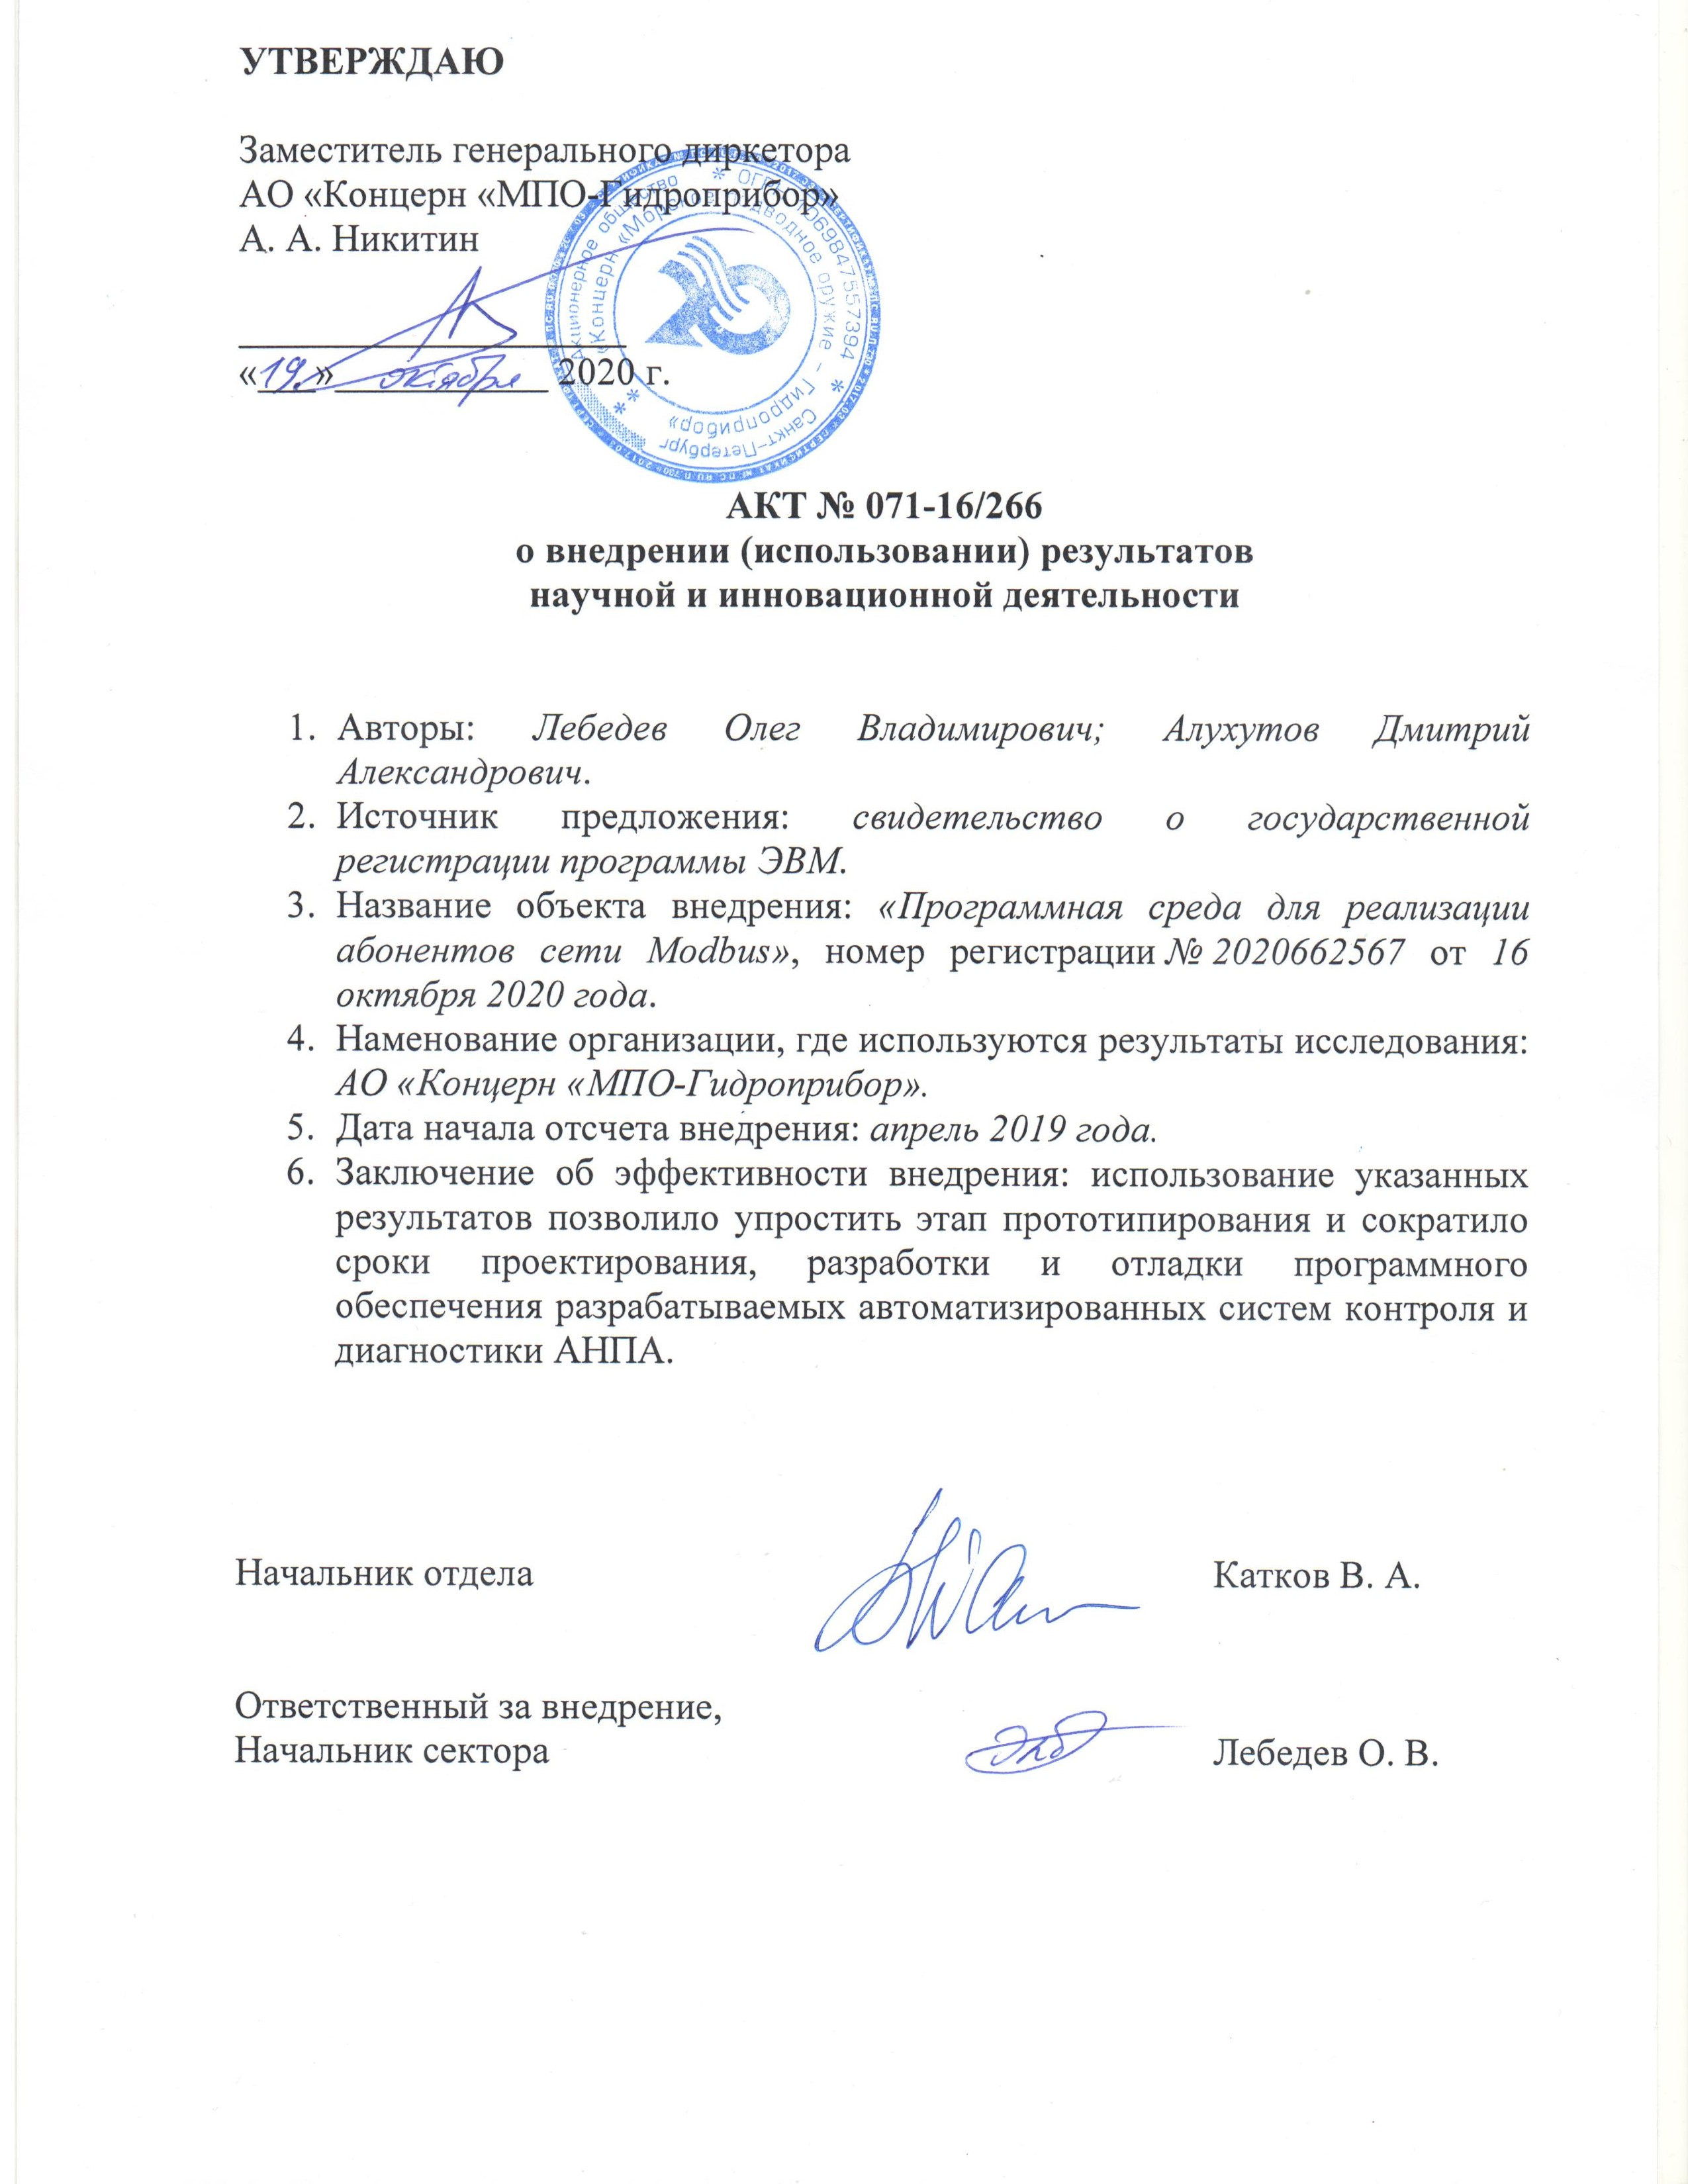
\includegraphics[height=.75\textheight]{implementation}
    \caption[Акт о внедрении]{Акт о внедрении на предприятии \leadingOrganizationTitle.}\label{app:fig:implementation}
\end{center}\end{figure}


\chapter{Дополнительные рисунки}\label{app:sec:figures}
\begin{figure}[hb!]\begin{center}
    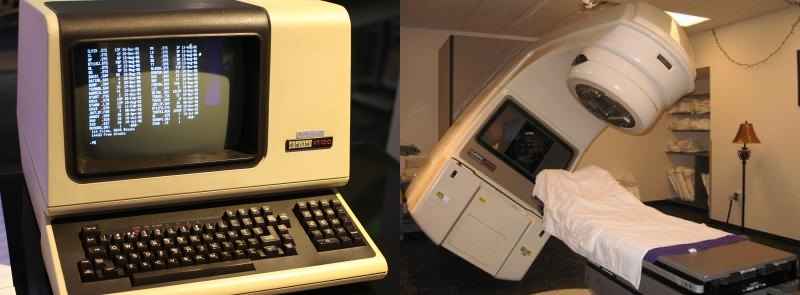
\includegraphics[width=.8\textwidth]{therac25-console}
    \caption[Therac 25]{Therac 25. Консоль оператора показана на рисунке \ref{app:fig:therac25_console}.}
        \label{app:fig:therac25}
    %
    \vspace{10mm}
    %
    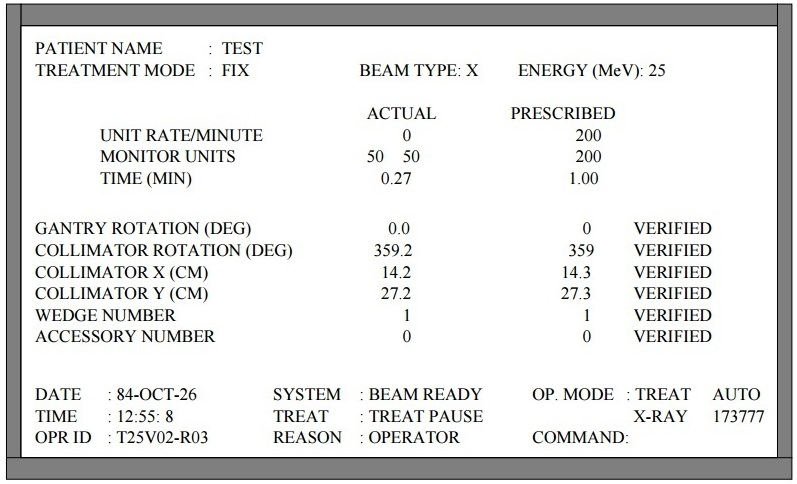
\includegraphics[width=.8\textwidth]{therac25-screenshot}
    \caption[Консоль Therac 25]{Консоль Therac 25.}\label{app:fig:therac25_console}
\end{center}\end{figure}

